\documentclass[10pt]{report}
\usepackage{graphicx}
\usepackage{hyperref}
\usepackage{float}
\usepackage[english]{babel}
\usepackage{graphicx}


\renewcommand\thesection{\arabic{section}}
\renewcommand\thesubsection{\thesection.\arabic{subsection}}

\newcommand*{\titleGM}{\begingroup % Create the command for including the title page in the document
\hbox{ % Horizontal box
%\hspace*{0.01\textwidth} % Whitespace to the left of the title page
\rule{1pt}{\textheight} % Vertical line
\hspace*{0.05\textwidth} % Whitespace between the vertical line and title page text
\parbox[b]{0.75\textwidth}{ % Paragraph box which restricts text to less than the width of the page

{\noindent\Huge\bfseries User Interface \\Design}\\[2\baselineskip] % Title
{\large \textit{Final submission}}\\[4\baselineskip] % Tagline or further description
{\Large \textsc{Arno De Witte}}\\
{\Large \textsc{Kwinten Pardon}}

\vspace{0.5\textheight} % Whitespace between the title block and the publisher
}}
\thispagestyle{empty}
\endgroup}

\begin{document}

\titleGM
\clearpage\setcounter{page}{1}

\section{Application Description}
The application focuses on students and professors at the university. This application allows for them to ask questions and give responses. They are able to log in into the application using their university credentials. Students are able to navigate through the courses they are registered for. Per course a student is able to see the questions asked by his fellow students and he's able to ask question of his own. A professor sees the courses he is responsible for. Per course the professor sees the questions asked by his students and is able to answer them. Due to these interactions, a knowledge base per course is formed. Professors can choose to close questions if they find that they are sufficiently answered. Because some questions might be irrelevant for other students, the student may choose to make a question private so that only the professor can see the question.

\section{Prototype}
A prototype has been developed as a web application. This choose was made as it seemed the most relevant for an actual working product. The prototype of our application can be found attached to this document. There is also a live version which can be found on \url{http://aropop.github.io/UIDproject/}. Note that the functionality of this prototype is written in JavaScript. Which means that when closing and reopening the page, all user data will be erased.\\
To use the application as a student (see section \ref{sec:Users}) the user should login using \emph{bad@student.be} or \emph{good@student.be}. Logging in as \emph{mathteacher@personel.be} will allow you to be the professor for the math course in the prototype.

\section{Users}\label{sec:Users}
The application is based on 2 existing user classes. It contains students who are taking courses on the one hand and professors in charge of said courses on the other. The application does not require a super user since the application is based in a university environment and all data should be imported from other already existing databases or applications.

\subsection{User Classes}

\subsubsection{Student}

\begin{tabular}{ | l | p{10cm} |}
\hline
\textbf{Type} & Primary User \\ \hline
\textbf{Usage frequency} & Daily Use \\ \hline
\textbf{Computer experience} & Novice \\ \hline
\textbf{Application familiarity} & From novice as first degree bachelor student to competent performer in second degree master student. Application shows familiarity's with other applications such as Pointcarre\\ \hline
\textbf{Usage} & discretionary\\ \hline
\textbf{Number of users} & 12.000+\\ \hline
\textbf{Motivation} & 
	\begin{itemize}
		\item Positive 
		\begin{itemize}
			\item eliminates the search for contact information
		\end{itemize}
	\end{itemize} \\ \hline
\textbf{tasks} & 
	\begin{itemize}
		\item Watch overview of courses (number of new questions / new answers per course)
		\item Watch overview of questions status per course (answered, follow-up question unanswered, unanswered)
		\item Ask a question regarding a course (public or private)
		\item Mark a question as answered (only if he is the original person who asked the question)
		\item Ask follow-up question
	\end{itemize} \\ \hline
\end{tabular}

\subsubsection{Professor}

\begin{tabular}{ | l | p{10cm} |}
\hline
\textbf{Type} & Primary User \\ \hline
\textbf{Usage frequency} & Daily Use \\ \hline
\textbf{Computer experience} & Novice \\ \hline
\textbf{Application familiarity} & Competent Performer due to similarities with other systems such as Pointcarre \\ \hline
\textbf{Usage} & Mandatory\\ \hline
\textbf{Number of users} & 700\\ \hline
\textbf{Motivation} & 
	\begin{itemize}
		\item Positive 
		\begin{itemize}
			\item Questions, separated by class instead of cluttered in email inbox
			\item Preventing duplicate questions by making a question public
		\end{itemize}
		\item Negative 
		\begin{itemize}
			\item Might prefer email
		\end{itemize}
	\end{itemize} \\ \hline
\textbf{tasks} & 
	\begin{itemize}
		\item Watch overview of courses (number off new questions, follow up questions per course)
		\item Watch questions per course (unanswered new, unanswered follow up question, answered)
		\item Filter questions (unanswered new, unanswered follow up question, answered)
		\item Change private question to public
		\item Answer (follow-up) question
		\item Discard question (refuse to answer)
	\end{itemize} \\ \hline
\end{tabular}

\subsection{User Models}

\begin{center}
	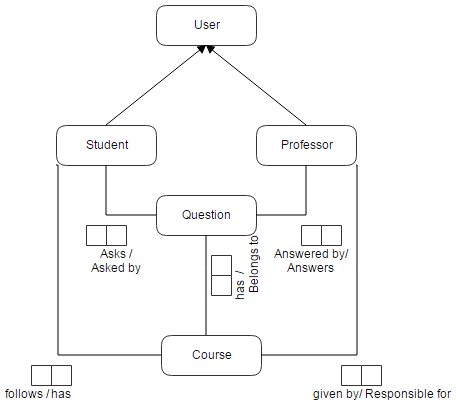
\includegraphics[scale=1]{img/orm.png}
\end{center}

\begin{itemize}
\item User has two subclasses, one for each user type
\item A student follows multiple courses
\item A student asks multiple questions
\item A professor answers multiple questions
\item A professor is in charge of multiple courses
\item A course is followed by multiple students
\item A course contains multiple questions
\item A course has multiple responsible professors
\item A question is related to a single course
\item A question can be asked by only one student
\item A question can be answered by only one professor

\end{itemize}

\subsection{Usability Requirements}
\begin{itemize}
	\item Users should be able to log in, within 10 seconds using their university credentials.
	\item Users should be able to navigate to the right course within 30 seconds.
	\item Students should be able to start the process of asking a question within 10 seconds. (Time on completing this task is dependant on the complexity of the question).
	\item Professors should be able to start the process of answering a question within 10 seconds. (Time on completing this task is dependant on the complexity of the question).
	\item Users should be able to find a question within 10 seconds. (only if they're already in the right course. If not time required to navigate to the right course should be included making it 40 seconds)
	\item Users should be able to change the status of a question instantly, provided the question already has been found.
	\item Users should be able to change the visibility of a question instantly, provided the question already has been found.
\end{itemize}

\section{CTT}
To model each possible task that is possible in our system we used ConcurTaskTrees (CTT). These were then further used in the development of the prototype.\\
Below in figure \ref{fig:cttTop} you can find the top level of the CTT. Attached to this document you can find each image as well as a global CTT.

\begin{figure}[H]
\centering
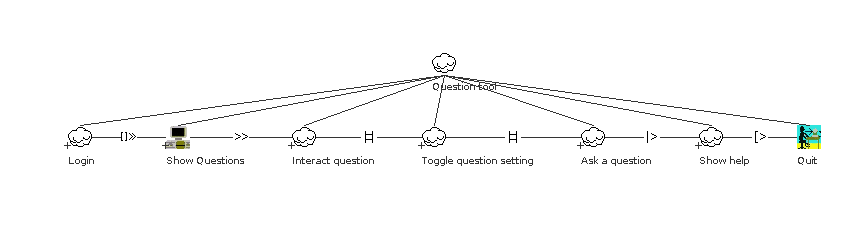
\includegraphics[scale=0.5]{../../ctt/ctttoplevel.png}
\caption{Top level CTT.}
\label{fig:cttTop}
\end{figure}
As seen there are 7 top level tasks. Before a user can do anything in our system, the user has to login. When the login is successful the users email will be passed on to the other tasks. When the login is successful the questions will be showed. Then all other tasks will be enabled. A user can stop using the application at any time which is modelled by the \emph{quit} task.\\
We will now discuss each task individually.\\

In figure \ref{fig:ctt1} CTT you can see the login task.
\begin{figure}[H]
\centering
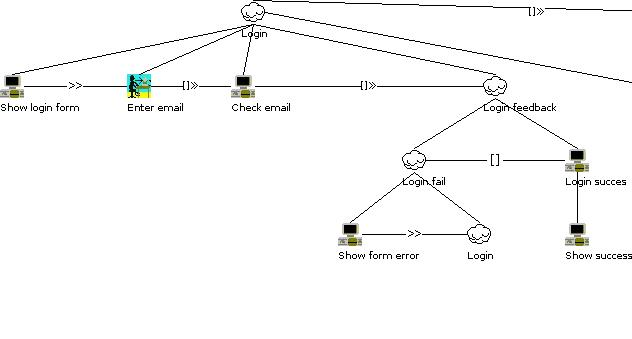
\includegraphics[scale=0.47]{../../ctt/ctt1.jpg}
\caption{Login CTT.}
\label{fig:ctt1}
\end{figure}
First the login form is displayed. The user should then provide his email address, which is then checked. Upon success the user gets a success message. Upon failure, the error is displayed on the login form and the user can try to correct this error and try to submit his or hers information again.\\

In figure \ref{fig:ctt2} the showing of questions, which happens after a user is logged in.
\begin{figure}[H]
\centering
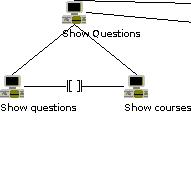
\includegraphics[scale=0.6]{../../ctt/ctt2.jpg}
\caption{Show questions CTT.}
\label{fig:ctt2}
\end{figure}
The showing of all questions is a combination of showing all courses and showing all questions. A user can then select a different course if necessary.\\

In figure \ref{fig:ctt3} the interaction with questions is modelled.
\begin{figure}[H]
\centering
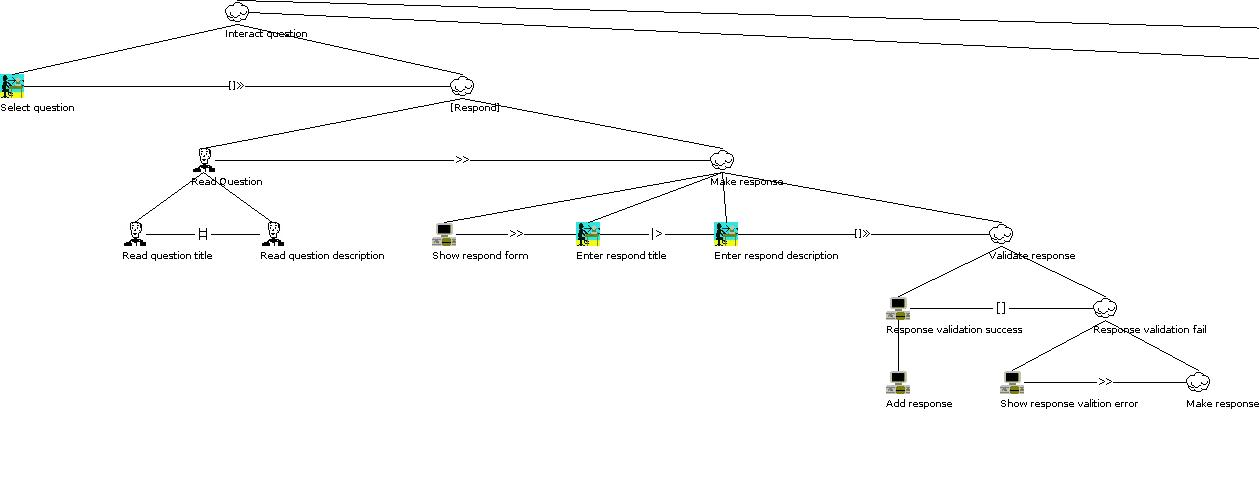
\includegraphics[scale=0.3]{../../ctt/ctt3.jpg}
\caption{Interact CTT.}
\label{fig:ctt3}
\end{figure}
A user can choose to select a question. This question (title and description) can then be read. A user can reply to a question by filling out the form (title and description), this form is then validated and the response is then posted. \\

In figure \ref{fig:ctt4} the toggling of settings. Two settings are available: the option to open or close a question and the option to make a question private or public. Private questions are only visible for the teacher and the asking user.
\begin{figure}[H]
\centering
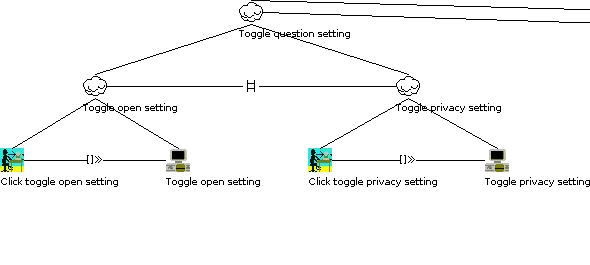
\includegraphics[scale=0.53]{../../ctt/ctt4.jpg}
\caption{Toggle settings CTT.}
\label{fig:ctt4}
\end{figure}
These toggles should be rather simple. A simple click (or similar interaction) should be enough.\\

The figure \ref{fig:ctt5} models the task of asking a question.
\begin{figure}[H]
\centering
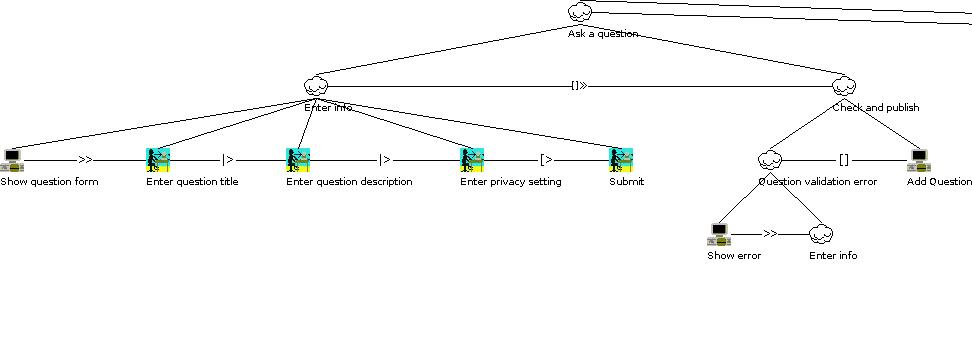
\includegraphics[scale=0.43]{../../ctt/ctt5.jpg}
\caption{Toggle CTT.}
\label{fig:ctt5}
\end{figure}
Asking a question is just a matter of showing the new question form, filling in the necessary information (title, description and whether or not this question should private then validating this form (same as for the other forms above).\\

To provide a help to users, the showing of an help overlay is modelled in figure \ref{fig:ctt6}.
\begin{figure}[H]
\centering
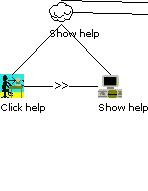
\includegraphics[scale=0.53]{../../ctt/ctt6.jpg}
\caption{Help CTT.}
\label{fig:ctt6}
\end{figure}
This can be done in a suspend-resume fashion from any of the other tasks, with the exception of the login. The user should should to open the help, after which it is displayed.



\section{Style Guide}
For our style guide we based ourselves upon the material design guidelines created by Google\footnote{\url{https://www.google.com/design/spec/material-design/introduction.html}}. These are design guidelines specifically made for use on all sorts of different screen sizes. It uses a flat simple design that aims to be intuitive. Implementation for these guidelines can be found in numerous of Google products and in a lot of other applications, both mobile and on the web.\\
These guidlines are also implemented in some web frameworks, we used material design lite which is implemented by google. We based this prototype upon one of the templates provided by default from this framework.\\

Below are some of the interaction as defined by our style guide:\\
\begin{itemize}

\item Standards for window interaction: Handled by the browser.
\item Standard window layout: A top bar with the title of the current page (equal to the current course in our application). This top bar should contain the main actions possible on the current page. In our prototype these are search and a action drop down menu. A menu bar containing the main pages (the different courses), information of the current user on top and if applicable a help button. This menu bar should be collapsed on devices with a small screen width.
\item Standards for buttons and menus: Buttons should have bright colour and if applicable an icon to indicate their action. If a default icon (material design provides a set of icons\footnote{\url{https://design.google.com/icons/}}) can not be found for the action, the button may contain text. For actions that add main content objects such as seen in the current screen, a so called FAB (floating action button) button should be provided in the bottom right of the screen. For toggles, icons or sliders can be used. When creating an item or for use in a form, sliders are used. When listing the action in an overview a icon should be used.\\
Menu's should be indicated with the 3 dot icon. They should drop down, have a white background and have their items as text. When all items of a menu can be illustrated with an icon, icons may be used. However this is not the case in the prototype.\\
Whenever using an icon, the usage of a tool tip (a small grey box with some helpful text that pops up when hovering over the icon) is highly recommended but not required. 
\item Standards for use of keyboard: When in a form, the tab key is used to go to the next item in the form. The enter key indicates that the user wants to commit his or hers input. These are standards widely used on the web.
\item Standards for text: In material design the roboto font is used\footnote{\url{https://www.google.com/fonts/specimen/Roboto}}. This font is used because it performs well on different screen sizes. The default size is 14 pixels for text. For titles the font size may very depending on which kind of title. The colour of the text depends on its background. For darker background (such as the sidebar) white or light grey text is used. When indicating additional information about a content object (for example the author of a question) it's recommended to use an italic font style to indicate that the text is a piece of meta information.
\item Standards for colour: Colour can be used to indicate the difference between areas. For example the difference in colour between the title of a question and the description or the difference between the main panel and the sidemenu. Items that should draw attention, such as the FAB, should have a bright colour.
\item Standards for user objects: The only relevant user object for this prototype is a question. Questions are listed in a list, each question should be initially collapsed to indicate it is not in use. When in the collapsed state, only the question title is visible. Users can however perform actions (toggle visibility, open/close) on them. When opening a question the description and potential responses become visible. Also if the question is open, the user gets the response form.
\item Standards for integration of information from other applications: Users can use the copy paste feature in their browser to copy text into the input fields.  
\end{itemize}


\section{Design Report}
\subsection{Problem Definition}
The goal of this project was to create a platform to enable students to ask questions in relation to a certain class they follow. Professors in turn would be able to answers these question.

We decided on 2 user classes, students and professor. You can read the user classes in detail in section \ref{sec:User_classes}

The tasks, as defined in section \ref{sec:CTT} consist of the following procedures

\begin{itemize}
\item Log in
\item Log out
\item View courses
\item View questions
\item Ask question
\item Answer question
\item Change visibility off question
\item Change status of question
\item Search for question
\end{itemize}

We were unable to complete the creation of the task models via the MARIA tool provided. When trying to download the task models, we were faced with a network error.

several iterations have gone over both the wireframes as the digital prototype. The prototype can be found running on http://aropop.github.io/UIDproject/ and the wireframes have been included as attachment 

\section{Evaluation report}
When designing this prototype we started out by sketching the design on paper. We tried to make the best possible model to fit our requirements. Then we created the wireframes. These are quite hard to iteratively improve, therefore we set out to create a working prototype as fast as possible. When we created the prototype we each evaluated the parts of the prototype each member had created. In this phase already some improvements were made. For example the email verification was improved by adding the support to just press enter.\\
In a second phase the prototype was send to another group for evaluation. There evaluation was very helpful as it provided an independent view on our prototype. The group pointed out some flaws in our prototype, such as the meaning of each icon and the fact that the placement of some buttons might be odd for new users. Therefor we added some tool tips and a help button which reveals an overlay that points to all features that might not be obvious to new users. Other small improvements were made based on this report which is included with this report.


\end{document}